\documentclass[a4paper,12pt]{article}
\usepackage{amsmath,amssymb,amsfonts,amsthm}
\usepackage{tikz}
\usepackage [utf8x] {inputenc}
\usepackage [T2A] {fontenc} 
\usepackage[russian]{babel}
\usepackage{cmap} 
\usepackage{ gensymb }
% Так ссылки в PDF будут активны
\usepackage[unicode]{hyperref}
\usepackage{ textcomp }
\usepackage{indentfirst}
\usepackage[version=3]{mhchem}

% вы сможете вставлять картинки командой \includegraphics[width=0.7\textwidth]{ИМЯ ФАЙЛА}
% получается подключать, как минимум, файлы .pdf, .jpg, .png.
\usepackage{graphicx}
% Если вы хотите явно указать поля:
\usepackage[margin=1in]{geometry}
% Или если вы хотите задать поля менее явно (чем больше DIV, тем больше места под текст):
% \usepackage[DIV=10]{typearea}

\usepackage{fancyhdr}

\newcommand{\bbR}{\mathbb R}%теперь вместо длинной команды \mathbb R (множество вещественных чисел) можно писать короткую запись \bbR. Вместо \bbR вы можете вписать любую строчку букв, которая начинается с '\'.
\newcommand{\eps}{\varepsilon}
\newcommand{\bbN}{\mathbb N}
\newcommand{\dif}{\mathrm{d}}

\newtheorem{Def}{Определение}


\pagestyle{fancy}
\makeatletter % сделать "@" "буквой", а не "спецсимволом" - можно использовать "служебные" команды, содержащие @ в названии
\fancyhead[L]{\footnotesize Квантовая физика}%Это будет написано вверху страницы слева
\fancyhead[R]{\footnotesize ФМХФ МФТИ}
\fancyfoot[L]{\footnotesize \@author}%имя автора будет написано внизу страницы слева
\fancyfoot[R]{\thepage}%номер страницы —- внизу справа
\fancyfoot[C]{}%по центру внизу страницы пусто

\renewcommand{\maketitle}{%
	\noindent{\bfseries\scshape\large\@title\ \mdseries\upshape}\par
	\noindent {\large\itshape\@author}
	\vskip 2ex}
\makeatother
\def\dd#1#2{\frac{\partial#1}{\partial#2}}


\title{1.3 \\ Эффект Мессбауэра}
\author{Егор Берсенев} 
\date{16 февраля 2017 г.}

\begin{document}
	
	\maketitle
	\section{Теоретическое введение}
		Эффект Мессбауэра --- это эффект переизлучения $\gamma$-квантов без генерации фононов. 
		Энергия, необходимая для смещения ядра составляет $10-30$ эВ. Поскольку энергия отдачи равна:
		\begin{equation}
		R = \frac{p^2}{M_n} = \frac{E^2_\gamma}{2M_nc^2}
		\end{equation}
		то ясно, что рассматриваемый случай реализуется только при больших энергиях $\gamma$-квантов. При испускании $\gamma$-квантов с $E<1$ МэВ энергия отдачи оказывается недостаточной для вырывания ядра из решетки, а импульс в той или иной форме передается всему кристаллу. Чаще всего энергия отдачи переходит в звуковые колебания решетки. На языке квантовой механики это значит, что энергия отдачи переходит квантам звуковых колебаний: фононам. Генерация фононов происходит тем легче, чем больше фононов уже имеется, т.е. при высоких температурах. При низких температурах этот процесс маловероятен. В этой ситуации большую роль начинает играть передача импульса отдачи всему кристаллу как целому. В формуле для энергии отдачи вместо массы ядра следует подставлять массу всего кристалла, вследствие чего энергия отдачи понижается на $10-20$ порядков, и становится пренебрежимо малой.
		Испускание и поглощение $\gamma$-квантов в твердых телах без рождения фононов носит название эффекта Мессбауэра. Теоретическое рассмотрение показывает, что вероятность эффекта определяется выражением:
		
		\begin{equation}
		f = \exp \left [-\frac{4\pi^2 \left<u^2\right> }{\lambda^2} \right]
		\end{equation}
		где $\left<u^2\right>$ --- среднеквадратичное смещение ядер в процессе тепловых колебаний, а $\lambda$ --- длина волны излучения.
		Видно, что вероятность упругого испускания и поглощения квантов уменьшается с температурой и ростом энергии перехода. Таким образом, расчет показывает, что эффект Мессбауэра ограничен областью малых энергий \linebreak$E\simeq200$ кэВ
		
		Эффект Мессбауэра изучается на ядрах олова $\mathrm{^{119}Sn}$ в $\mathrm{BaSnO_3}$. Гамма-излучение пропускается через резонансный поглотитель. Там происходит взаимодействие квантов излучения как с атомными электронами за счет фотоэффекта и эффекта Комптона, так и с ядрами атомов. Поэтому интенсивность:
		\begin{equation}
			\exp\left[-n_e\sigma_e\right]\exp\left[-nf\sigma(E)\right]
		\end{equation}
		Сечение резонансного поглощения имеет лоренцевскую форму кривой(формула Брейта-Вигнера)
		\begin{equation}
			\sigma(E) \sim \frac{\left(\Gamma/2\right)^2}{\left(E-E_0\right)^2 + \left(\Gamma/2\right)^2}
		\end{equation}
		Здесь $E_0$ --- энергия ядерного перехода, а $\Gamma$ --- естественная ширина линии.
		Для источника и поглотителя, находящихся в разных химических соединениях, максимум резонансного поглощения смещается относительно нулевой скорости на величину
		\begin{equation}
			v = \frac{\Delta E}{E}c
		\end{equation}
		Обычно в опыте по резонансному поглощению определяется величиной <<амплитуды>> эффекта
		\begin{equation}
			\eps(v) = \frac{N(\infty)-N(v)}{N(\infty)-N_f}
		\end{equation}
		где $N(v)$ --- скорость счёта квантов, прошедших через поглотитель при некоторой скорости $v$, $N(\infty)$ --- скорость счёта квантов при достаточно большой скорости, когда резонансное поглощение отсутствует, $N_f$ --- скорость счёта радиоактивного фона. Величина $\eps(v)$ является относительной величиной, и не зависит ни от активности, ни от величины поглощения излучения электронами.
		
		\section{Экспериментальная часть}
			Снимем спектры поглощения.
			\begin{figure}[h!]
				\centering
				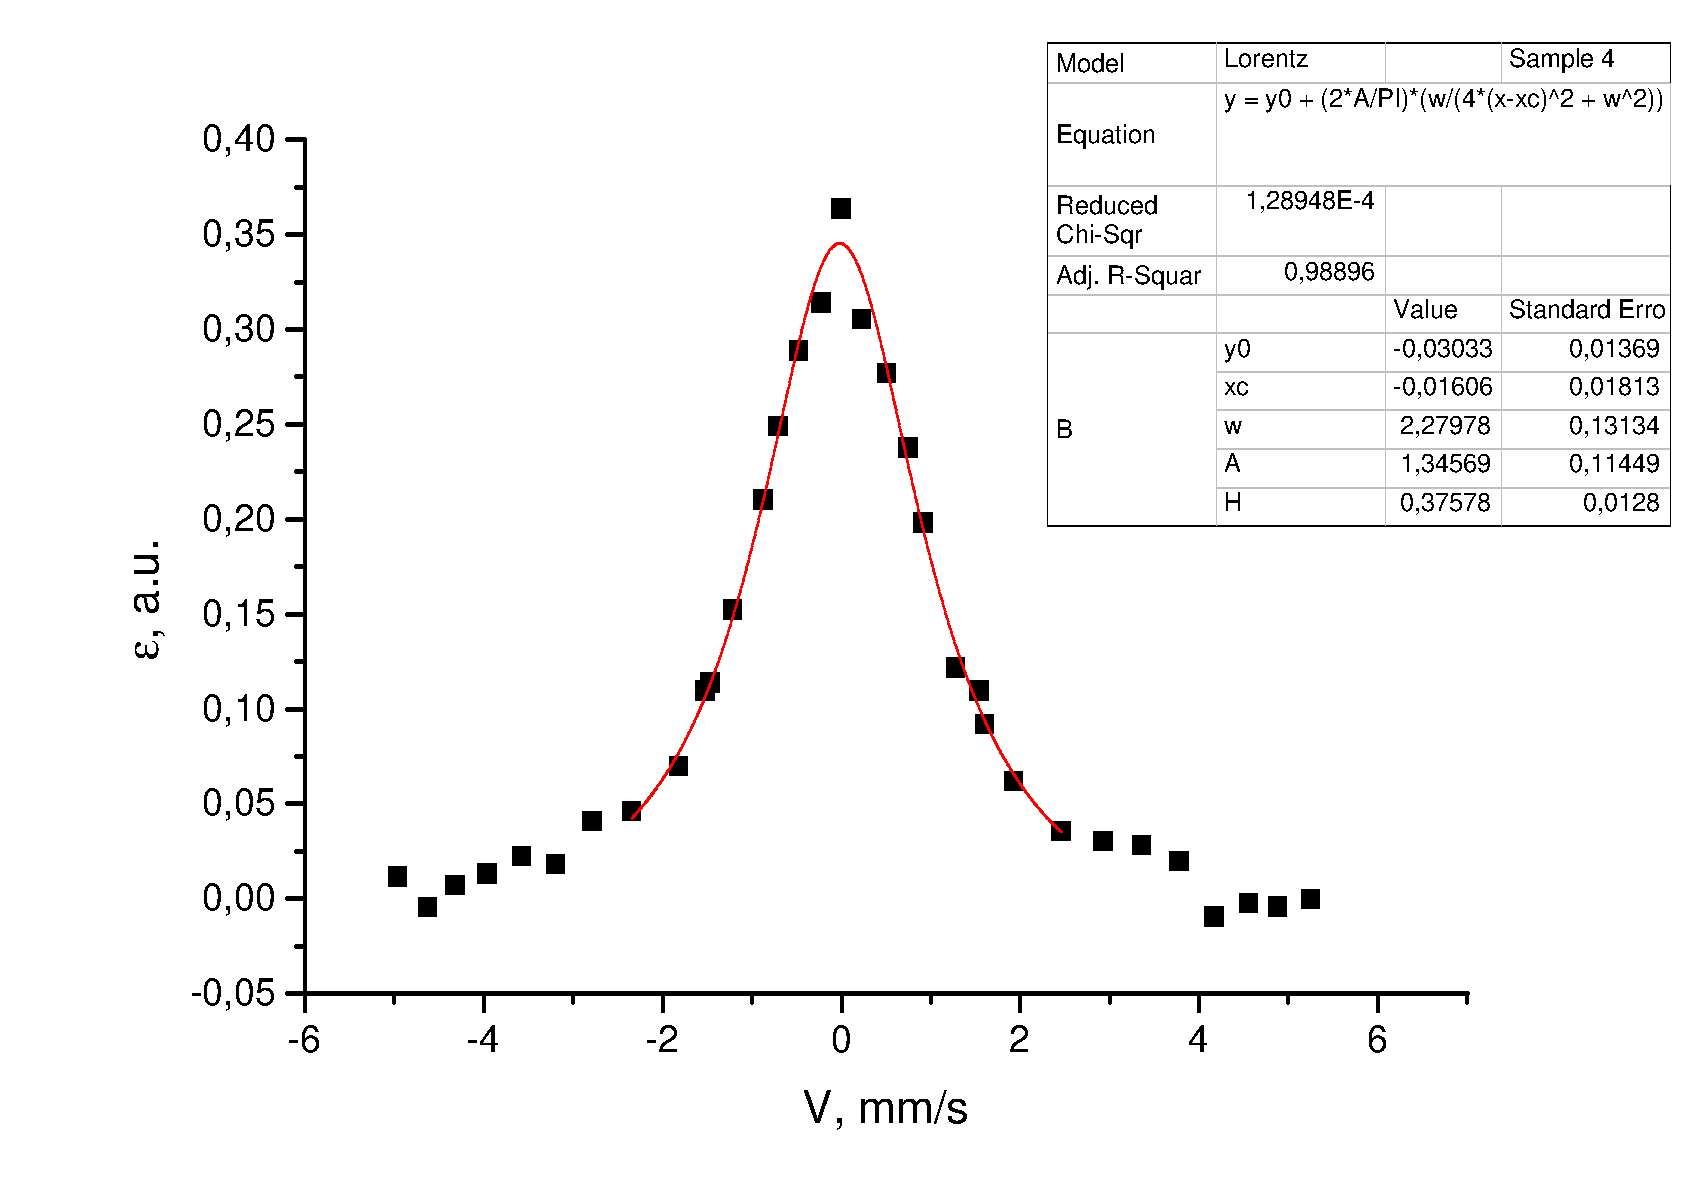
\includegraphics[width=1.1\linewidth]{sample4}
				\caption{Спектр поглощения образца 4}
			\end{figure}
			
			\begin{figure}[h!]
				\centering
				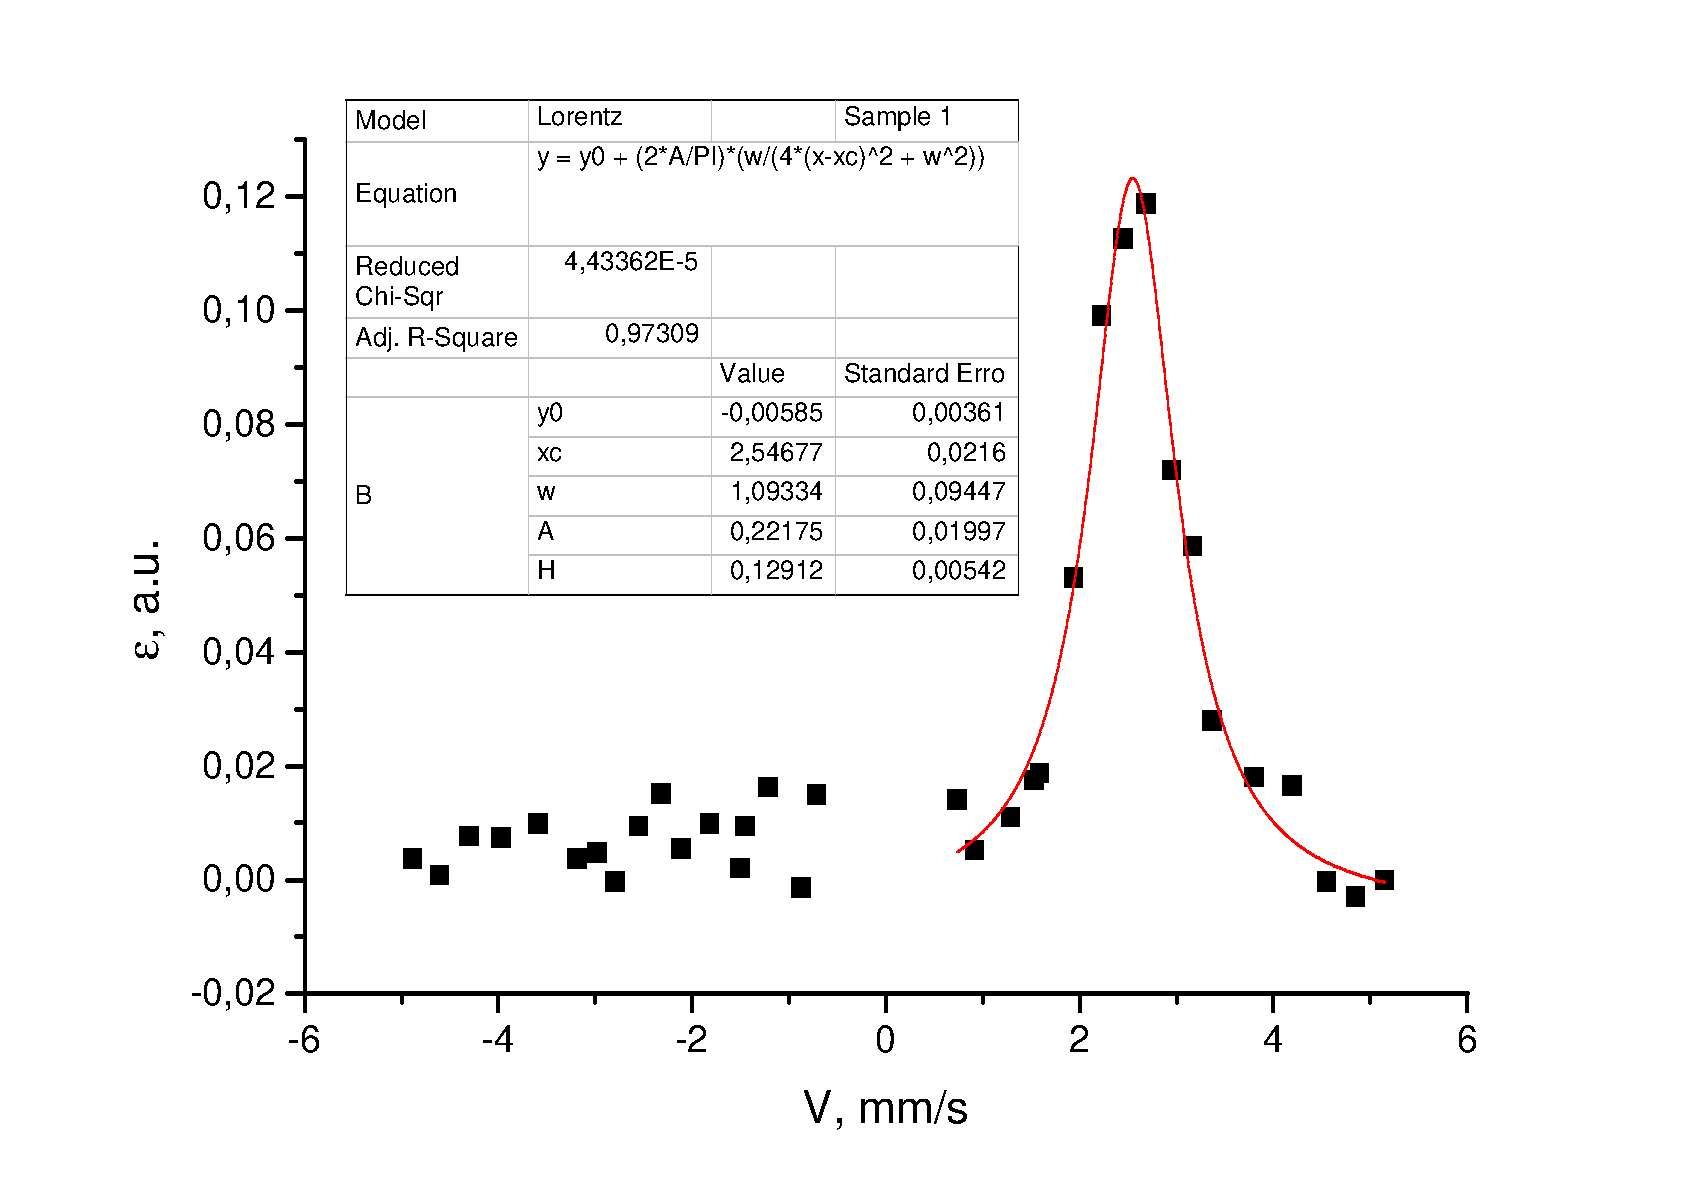
\includegraphics[width=0.95\linewidth]{sample1}
				\caption{Спектр поглощения образца 1}
			\end{figure}
			
			\begin{figure}[h!]
				\centering
				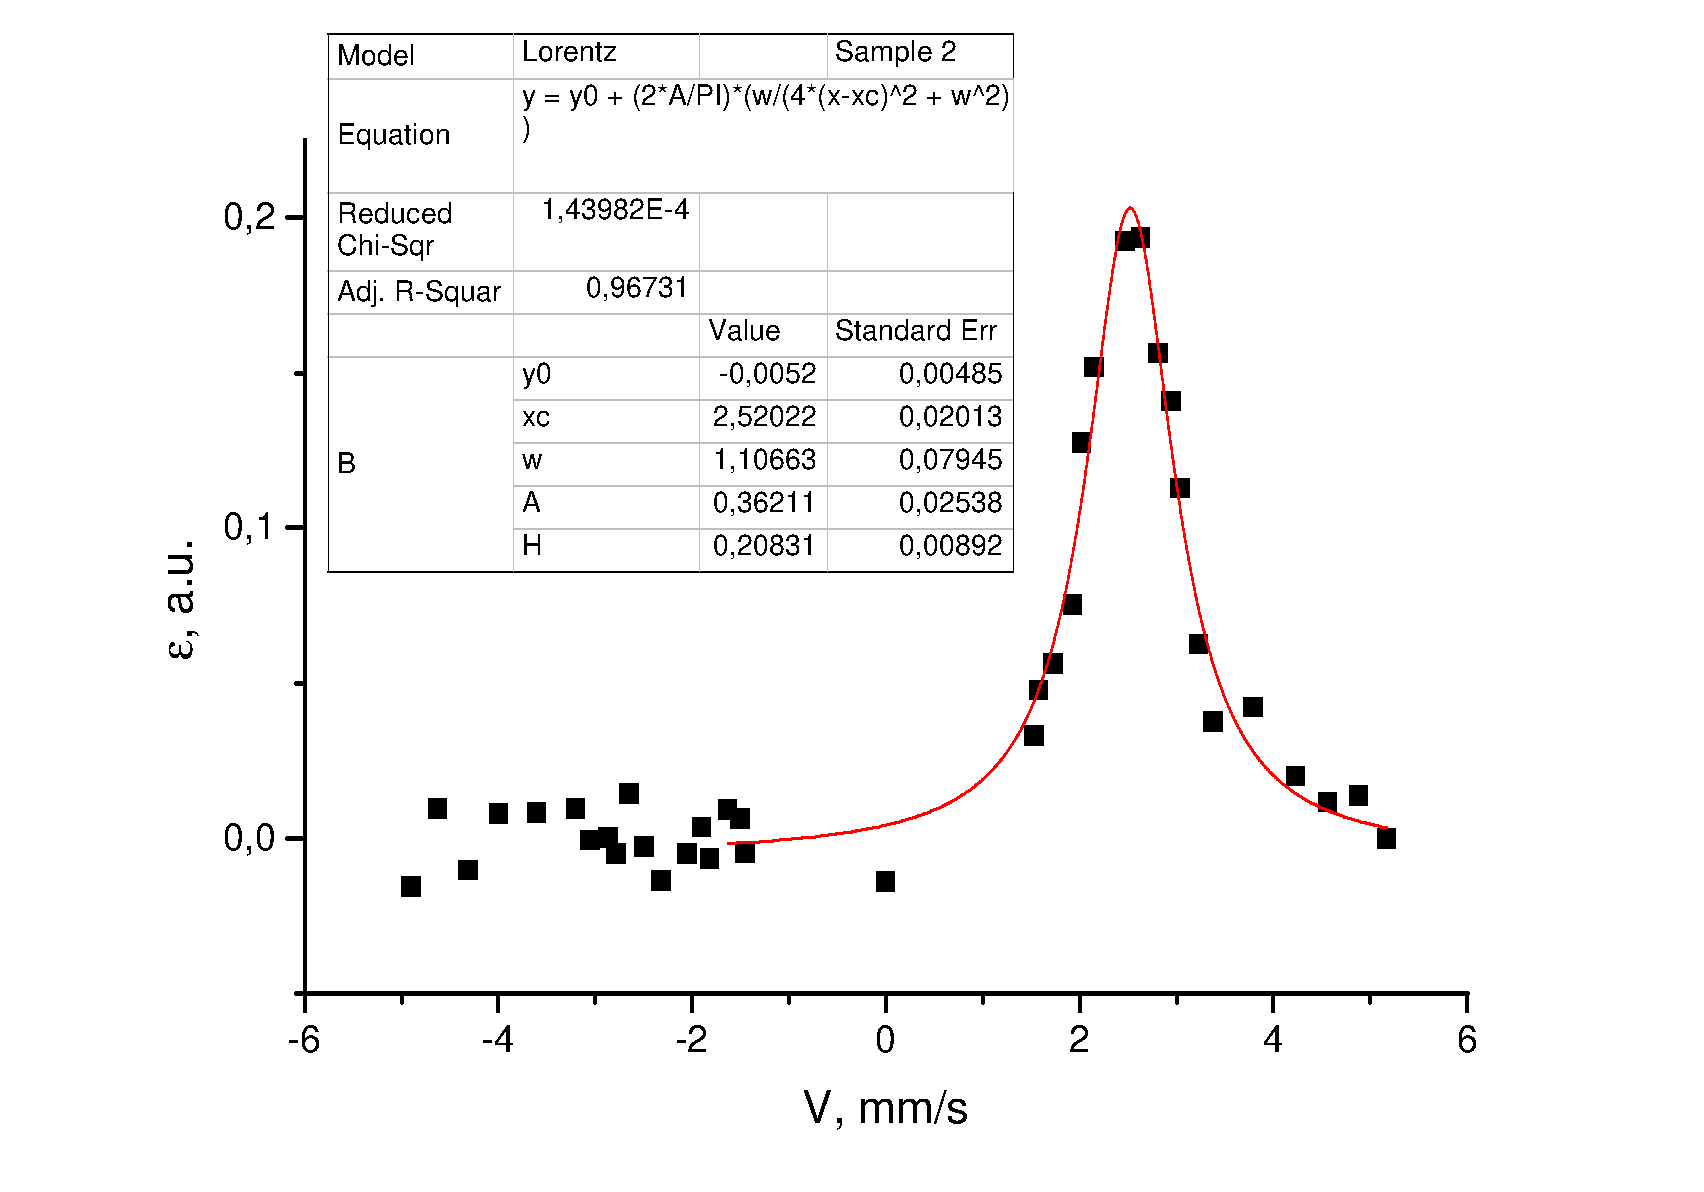
\includegraphics[width=0.95\linewidth]{sample2}
				\caption{Спектр поглощения образца 2}
			\end{figure}
		
		\newpage
		
		Пересчитаем ширину линии и химический сдвиг из мм/с в эВ. Естественная ширина линии $\Gamma = 3\cdot10^{-8}\mathrm{eV}$. В таблице же указана двойная ширина линии $2\Gamma$
		
		\begin{table}[h!]
			\centering
			\caption{Результаты эксперимента}
			\label{my-label}
			\begin{tabular}{|l|l|l|l|}
				\hline
				& 1 & 2 & 4 \\ \hline
				$w, \mathrm{mm/s}$ & 1.09  & 1.11  & 2.28  \\ \hline
				$w, \mathrm{eV}\cdot 10^{-8}$   & 9.2  & 9.4  & 19.3  \\ \hline
				$\dif x, \mathrm{mm/s}$      & 2.55  & 2.52  & -0.02  \\ \hline
				$\dif x, \mathrm{eV}\cdot 10^{-8}$      & 21.6  & 21.3  &  -0.17 \\ \hline
			\end{tabular}
		\end{table}
	
	
	Попробуем приблизить экспериментальные данные гауссовой кривой:
	\begin{figure}[h!]
		\begin{center}
			\begin{minipage}{0.32\textwidth}
				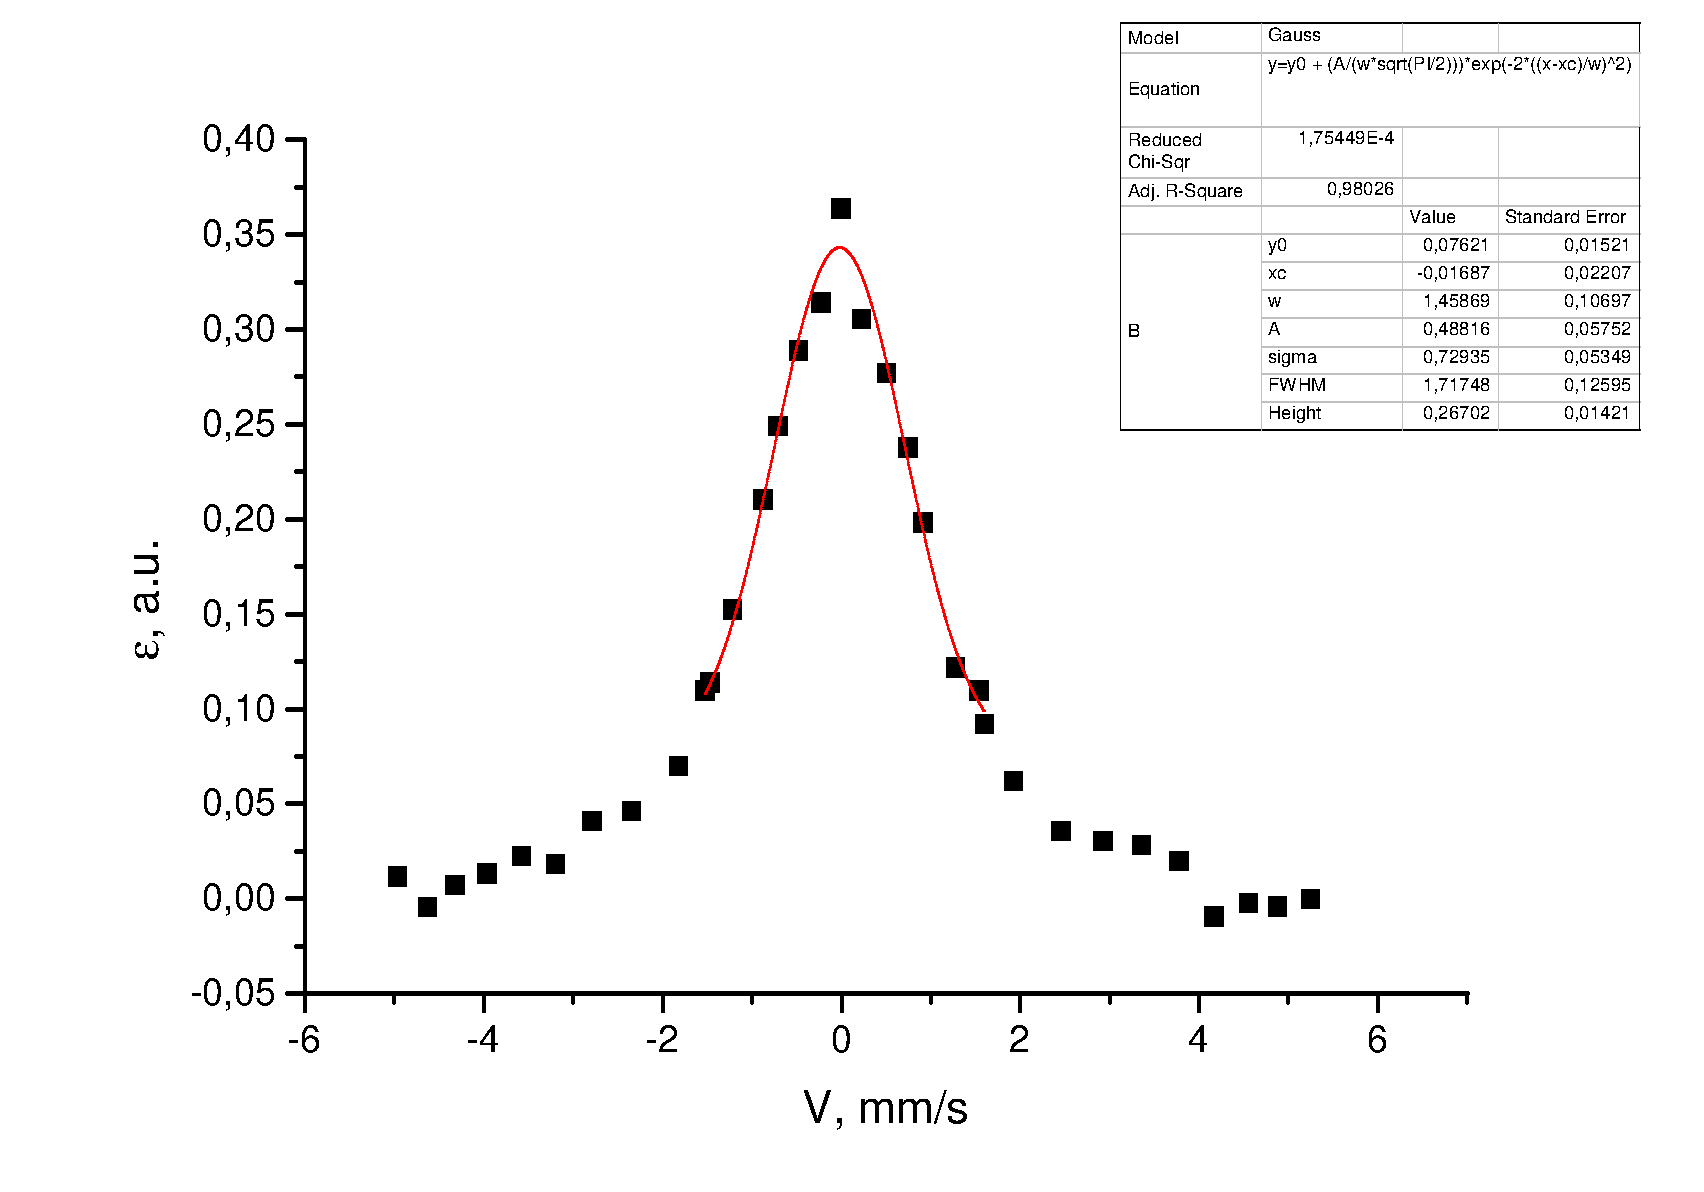
\includegraphics[width=\textwidth]{sample1_g}
			\caption{Образец 1}
		\end{minipage}
		\hfill
		\begin{minipage}{0.32\textwidth}
			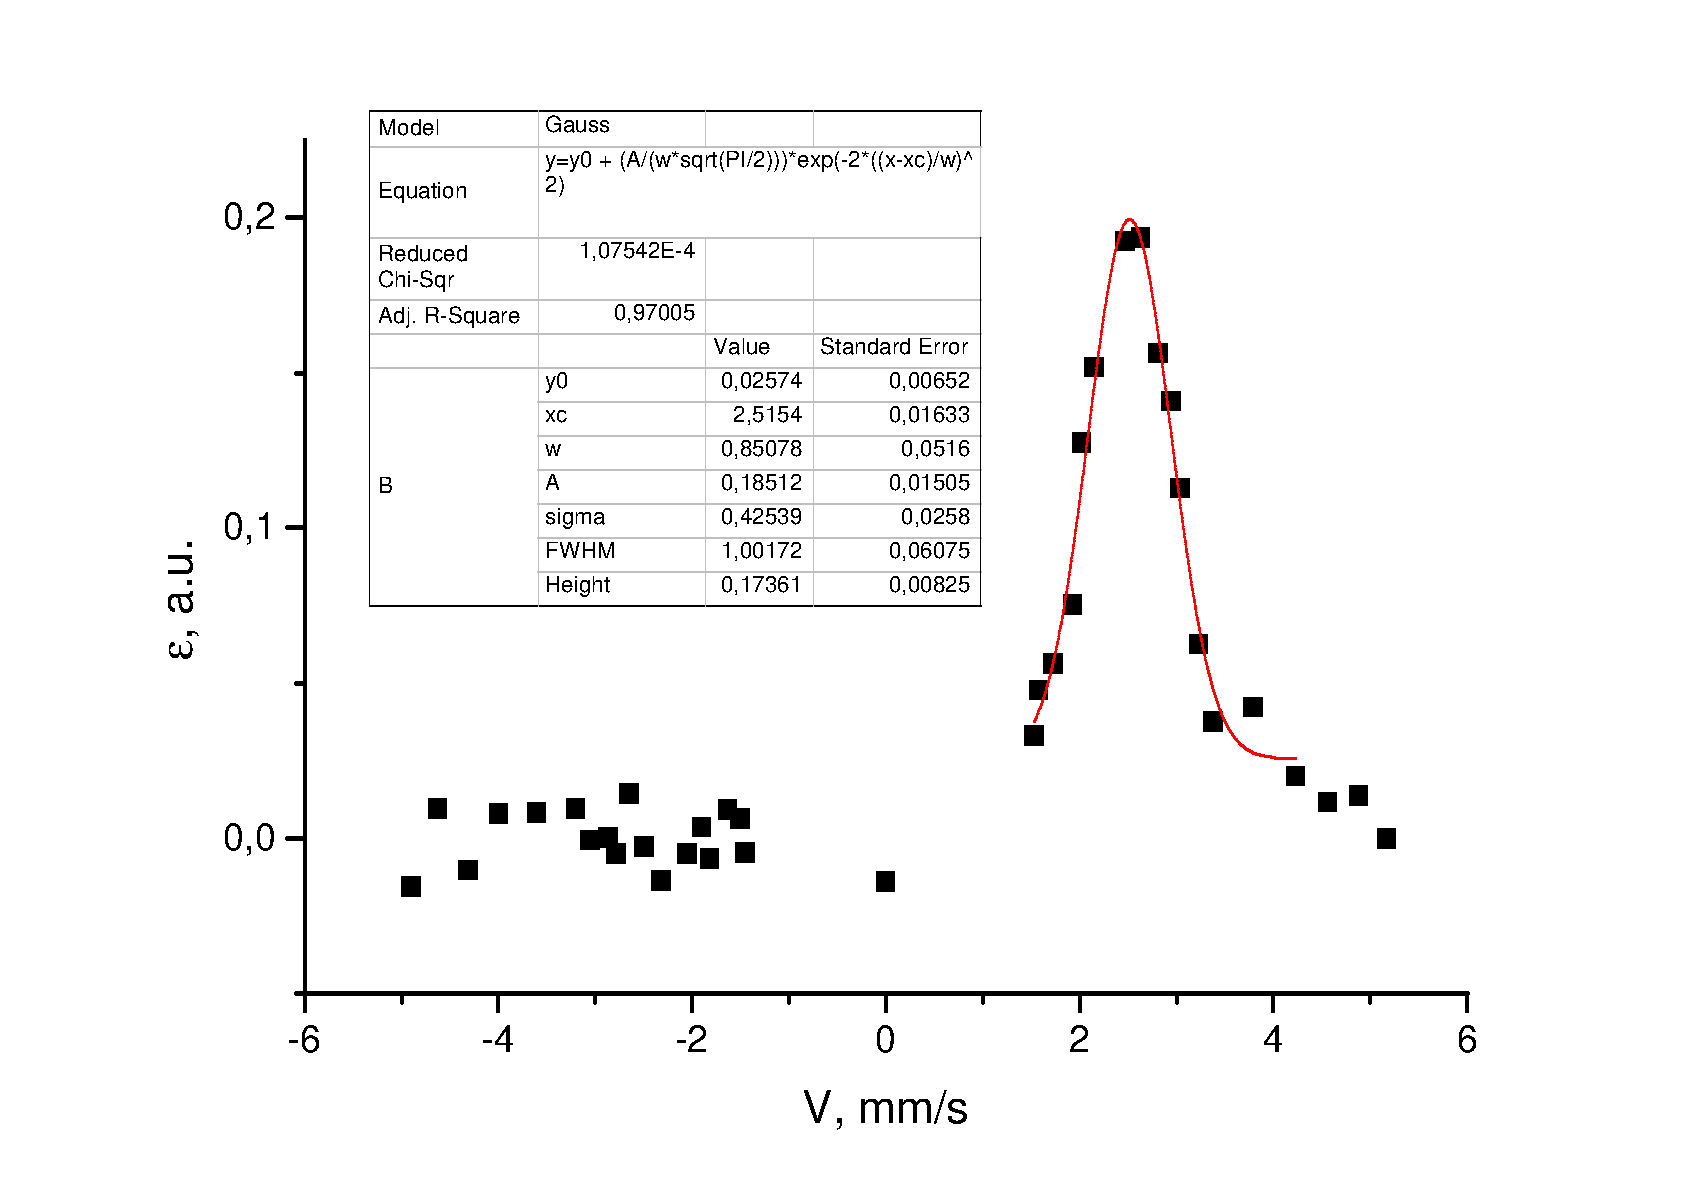
\includegraphics[width=\textwidth]{sample2_g}
			\caption{Образец 2}
		\end{minipage}
		\hfill
		\begin{minipage}{0.32\textwidth}
			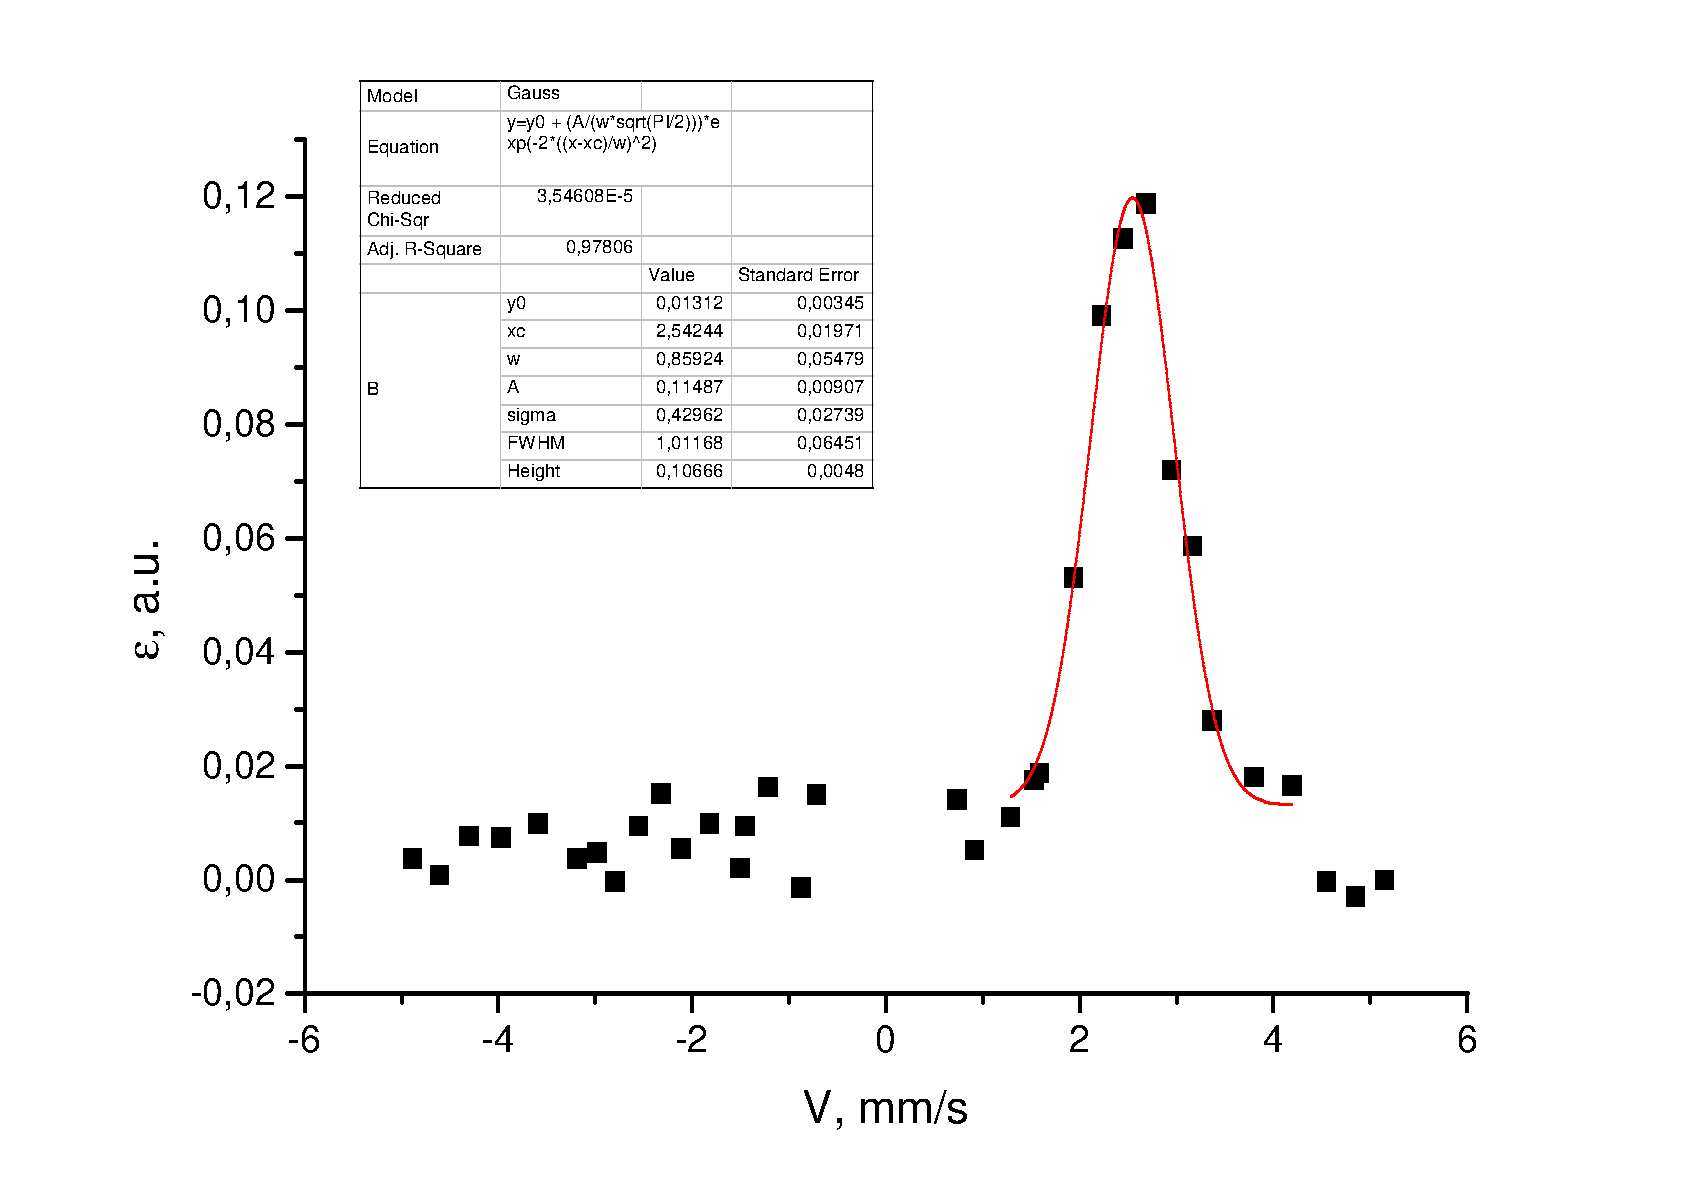
\includegraphics[width=\textwidth]{sample4_g}
			\caption{Образец 4}
		\end{minipage}
	\end{center}
	\end{figure}
		$\chi^2$ показывает, что в некоторых случаях гауссова кривая лучше приближает экспериментальные данные. Почему так происходит --- не совсем ясно, но основной проблемой считаю фактор кривых рук.
		
	\section{Вывод и обсуждение результатов}
		Эффект резонансного поглощения $\gamma$-квантов может применяться для исследования структур, содержащих определенные изотопы. Поскольку мессбауэровская линия очень узка, то для того, чтобы резонанс нарушился необходима ничтожная скорость порядка мм/с. Основными причинами уширения линии можно считать нарушение равномерности движения образца, т.к. не всегда время прохождения линейного участка было меньше, чем время измерения и уширение, связанное с вибрациями установки, которые могли произойти по любой причине, включая проходящих мимо людей.
\end{document}


